% !TEX program = pdflatex
\documentclass[11pt,a4paper]{article}

% === PACKAGES (house style, mirrored from learned-bloom-filter) ===
\usepackage[utf8]{inputenc}
\usepackage[T1]{fontenc}
\usepackage{lmodern}
\usepackage[margin=1in]{geometry}
\usepackage{setspace}
\usepackage{parskip}
\usepackage{graphicx}
\usepackage{float}
\usepackage{booktabs}
\usepackage{amsmath}
\usepackage{amssymb}
\usepackage{hyperref}
\usepackage{listings}
\usepackage{xcolor}
\usepackage{caption}
\usepackage{subcaption}
\usepackage{tikz}
\usepackage{pgfplots}
\pgfplotsset{compat=1.18}

% === CODE LISTING STYLE ===
\definecolor{codegreen}{rgb}{0,0.6,0}
\definecolor{codegray}{rgb}{0.5,0.5,0.5}
\definecolor{codepurple}{rgb}{0.58,0,0.82}
\definecolor{backcolour}{rgb}{0.95,0.95,0.92}

\lstdefinestyle{mystyle}{
    backgroundcolor=\color{backcolour},
    commentstyle=\color{codegreen},
    keywordstyle=\color{magenta},
    numberstyle=\tiny\color{codegray},
    stringstyle=\color{codepurple},
    basicstyle=\ttfamily\footnotesize,
    breakatwhitespace=false,
    breaklines=true,
    captionpos=b,
    keepspaces=true,
    numbers=left,
    numbersep=5pt,
    showspaces=false,
    showstringspaces=false,
    showtabs=false,
    tabsize=2
}
\lstset{style=mystyle}

% === TITLE INFO ===
\title{
    \vspace{-2em}
    \rule{\textwidth}{1pt}\\[0.5em]
    \textbf{ReDoS Safe-Regex Harness for Python}\\[0.3em]
    \large Measuring Real Timing and Proving Atomic-Group Fixes on Five CVE-Grounded Patterns\\[0.5em]
    \rule{\textwidth}{1pt}
}
\author{
    Ashay Kushwaha\\
    \textit{CypherLabs Open Research}\\
    \texttt{https://github.com/AshayK003/redos-harness}
}
\date{September 2026}

\begin{document}

\maketitle

\begin{abstract}
CPython is the only major regular-expression engine with no ReDoS defense: a 2024--2025 systematization of knowledge rates Rust and Go safe, JavaScript, Ruby, Java, and C\# partially defended, and Python ``not safe.'' Static checkers flag patterns without measuring real cost, and no single tool catches every evil pattern; dynamic fuzzers target other engines or cost thousands of CPU-hours. We present a fast standard-library-only Python harness that times five CVE-grounded patterns on pump strings, fits log-log growth exponents (linear / polynomial / exponential), auto-rewrites with Python 3.11+ atomic groups and possessive quantifiers, and re-times to prove each fix under a strict accept-rule (benign verdicts byte-identical AND growth class linear, both re-measured). On CPython 3.12: one exponential CVE pattern is fixed and proven linear, one suspect-shaped pattern is correctly classified clean (no false positive), and four cases are honestly reported unfixed with measured causes. Along the way we find that a published vendor proof-of-concept does not reproduce (0.0\,ms), and that possessive quantifiers alone cannot fix search-mode scanning. Every number regenerates with one command.
\end{abstract}

\vspace{1em}
\noindent\textbf{Keywords:} ReDoS, regular expressions, CPython, atomic groups, dynamic analysis, vulnerability measurement

\newpage
\tableofcontents
\newpage

\section{Introduction}

Copy-pasted validation regexes plus a backtracking engine equal super-linear blowup on crafted input. Email, URL, and cookie parsing via decades-old patterns remains the default in Python codebases, and Python's \verb!re! backtracks. The consequences are not theoretical: a single super-linear pattern caused global outages at Stack Overflow (2016) and Cloudflare (2019), and five recent CVEs---in CPython itself, pydantic, sqlparse, tornado, and Black---trace to exactly this failure mode.

The tooling landscape has two halves that never meet. Detection tooling (static AST checkers, dynamic fuzzers, hybrid frameworks) reports \textit{whether} a pattern is evil. Nothing ships the other half: a \textit{verified fix} with timing proof. The 2024 systematization of knowledge in this area states the open challenge directly: future work should ``support engineers in migrating to defended engines.'' Meanwhile Python 3.11 quietly shipped the fix primitive---atomic groups \verb!(?>...)! and possessive quantifiers---with zero guidance on which rewrite fixes which real-world pattern.

This report presents a harness that closes the loop on a frozen, CVE-grounded corpus: detect by measurement, rewrite with atomic constructs, and prove the fix by re-measurement. Our contributions:

\begin{itemize}
    \item A frozen v1 corpus of 6 entries across 5 real CVEs, each reproduced on CPython 3.12 with advisory-linked patterns and benign accept/reject strings.
    \item A standard-library-only timing harness (subprocess isolation, timeout-as-data, log-log exponent fitting) with a strict accept-rule for fixes.
    \item Measured results: 1 proven fix (exponential to linear), 1 clean control (no false positive), 4 honestly unfixed cases with measured causes.
    \item Two negative results worth reporting: a published vendor proof-of-concept that does not reproduce, and a possessive-quantifier fix attempt that wins constants but not complexity class.
\end{itemize}

\section{Background and Related Work}

\subsection{Python is the exposed engine}

The systematization of knowledge on ReDoS (34 papers, 2015--2024, published at ASIACCS'25 with a full artifact) surveys nine production regex engines for realized defenses. Rust and Go are safe (Thompson-style simulation); JavaScript, Ruby, C\#, and Java are partially defended (memoization, caching, timeouts, opt-in non-backtracking modes); Perl and PHP cap resources. \textbf{CPython has no defense of any kind} and is rated ``not safe.'' Every other major runtime shipped mitigation; Python did not. That asymmetry is the reason a Python-specific harness matters: findings from JS/Java tooling do not transfer to an engine with no safety net.

\subsection{Detection: static, dynamic, hybrid}

Detection research splits three ways. \textit{Static} approaches (safe-regex star-height heuristics, RXXR2 automata analysis, Rexploiter vulnerable-structure identification, plus industry linters and CodeQL queries) are fast but trade precision against recall, and cannot reason about all extended features such as backreferences. \textit{Dynamic} approaches (SDL Regex Fuzzer, ReScue's genetic search, SlowFuzz, REGULATOR's instrumented fuzzer) time real engines and eliminate false positives by construction, but are slow---ReScue averages 18\,s per pattern, REGULATOR's full evaluation cost $\sim$1000 CPU-hours---and were built around Java/JavaScript engines. \textit{Hybrid} approaches (ReDoSHunter at 100\% precision and recall on 37,651 patterns, NFAA, Revealer, RENGAR) combine both, but stop at detection: they output a verdict and an attack string, never a repaired pattern. A 2025 independent comparison of nine tools over twelve evil patterns found that no single tool catches everything, which is why our harness measures wall-clock behavior on the actual target engine instead of trusting any single detector's verdict.

\subsection{Python 3.11 atomic groups}

CPython 3.11 (bpo-433030) added atomic grouping \verb!(?>...)! and possessive quantifiers (\verb!*+!, \verb!++!, \verb!?+!, \verb!{m,n}+!). An atomic group commits to its first successful match and discards all backtracking points within itself, which is precisely the mechanism that converts exponential backtracking into a single linear pass---\textit{when} the first greedy path is also the correct one. That conditional is doing real work, and no published guidance maps it onto real CVE patterns. Our rewrite rules are deliberately narrow, and every candidate must survive re-measurement on benign inputs; Section~\ref{sec:discussion} shows a case where the obvious atomic rewrite is correctly rejected.

\subsection{The five CVEs}

Table~\ref{tab:corpus} lists the corpus. Each pattern was extracted from the upstream fix diff (not from prose descriptions, which we show in Section~\ref{sec:discussion} to be unreliable): Black's tab-expansion regex (fix commit \verb!f000936!), pydantic's email regex (commit \verb!59d8f38!), sqlparse's string lexer (commit \verb!c457abd!), tornado's cookie unquoter (commit \verb!d5ba4a1!), and CPython's tarfile header patterns (commit \verb!34ddb64!). Notably, upstream fixed Black, pydantic, tornado, and tarfile \textit{without} repairing any regex (string ops, length caps, single-pass restructures); only sqlparse repaired the pattern itself. Our atomic rewrites are therefore positioned as the \textit{alternative} fix, and the report says so wherever it matters.

\section{Methodology}

\subsection{Harness design}

The harness (\verb!harness.py!, standard library only: \verb!re!, \verb!time!, \verb!multiprocessing!, \verb!json!, \verb!statistics!) has three pieces. First, a \textit{pump generator} builds inputs as prefix + core$\times k$ + suffix at five doubling sizes per entry. Second, \textit{timing} runs each case in a worker \textit{process} (never a thread: a catastrophically backtracking match cannot be interrupted under the GIL) with a hard 15\,s timeout. A timeout is recorded as data, never swallowed---it is the strongest signal in the table. Third, \textit{benign checking} asserts every accept string matches and every reject string does not, comparing match/no-match verdicts only.

Two engineering details matter. Byte-oriented entries (tarfile) coerce str patterns to bytes rather than failing silently---a str-pattern-on-bytes input raises \verb!TypeError!, which an early version of the harness caught and mistimed at $\sim$0\,ms; the coercion plus a regression note fixed it. Timer resolution is handled by a noise floor: sub-millisecond ceilings read as linear, since no denial-of-service lives below a millisecond inside a 16$\times$ size sweep.

\subsection{Growth fitting}

For each entry we fit a log-log slope of wall time versus input size (ordinary least squares via \verb!statistics.linear_regression!): slope $\approx$ 1 is linear, $\approx$ 2 is quadratic, $\gg$ 2 is exponential. Timeout past the first length classifies as exponential directly---an attacker only needs the small input. Thresholds (1.6 / 2.5) are documented in code; Section~\ref{sec:results} shows every fitted slope landing where theory predicts (0.76--3.05 with the matching class), which is the calibration evidence.

\subsection{Accept-rule for fixes}

The rewriter (\verb!rewriter.py!) proposes candidates from a small conservative rule set (nested-plus to possessive, star-group to atomic wrap). A candidate is accepted \textit{if and only if} benign verdicts are byte-identical \textit{and} the growth class drops to linear, both re-measured---never inferred. A rule that proposes a constant-only win, or that alters any benign verdict, is rejected (one such rule was tried and deleted during development; Section~\ref{sec:discussion}).

\subsection{Corpus and freeze policy}

\verb!corpus.json! v1 is frozen: 6 entries across 5 CVEs, each with the exact pattern, match method, pump recipe, benign strings, advisory link, fix-commit link, and the upstream fix kind. Additions bump the version and re-run everything. Table~\ref{tab:corpus} summarizes it.

\begin{table}[H]
\centering
\caption{Frozen v1 corpus. All patterns extracted from upstream fix diffs and reproduced on CPython 3.12.10.}
\label{tab:corpus}
\begin{tabular}{@{}llll@{}}
\toprule
Entry & CVE & Pattern (method) & Upstream fix \\
\midrule
black-tabs & 2024-21503 & \verb!\s*\t+\s*(\S)! (match) & regex removed \\
pydantic-email & 2024-3772 & \verb!([\w ]*?) *<(.*)> *! (fullmatch) & length cap \\
sqlparse-string & 2023-30608 & string alternation (match) & pattern repaired \\
tornado-unquote & 2024-52804 & repeated \verb!.search! loop (driver) & single-pass sub \\
tarfile-pax & 2024-6232 & \verb!(\d+) ([^=]+)=! (match) & single-pass parser \\
tarfile-hdrcharset & 2024-6232 & \verb!\d+ hdrcharset=...! (search) & single-pass parser \\
\bottomrule
\end{tabular}
\end{table}

\section{Results}
\label{sec:results}

One command (\verb!python report.py!) regenerates Table~\ref{tab:results} and Figure~\ref{fig:growth}. Numbers below are the fresh-clone verification run (Section~\ref{sec:repro}).

\begin{table}[H]
\centering
\caption{Before/after benchmark (15\,s per-case timeout). Slopes are fitted log-log exponents.}
\label{tab:results}
\begin{tabular}{@{}llll@{}}
\toprule
Entry & Before (5 sizes) & Slope & Verdict \\
\midrule
black-tabs & 56ms $\to$ 385ms $\to$ 3.3s $\to$ T $\to$ T & 2.91 & UNFIXED \\
pydantic-email & 23ms $\to$ 85ms $\to$ 367ms $\to$ 1.6s $\to$ 6.1s & 2.03 & UNFIXED \\
sqlparse-string & 0.2ms $\to$ 254ms $\to$ T $\to$ T $\to$ T & --- & FIXED linear \\
tornado-unquote & 336ms $\to$ 1.3s $\to$ 5.0s $\to$ T $\to$ T & 1.96 & driver, measured \\
tarfile-pax & $\le$0.4ms throughout & 0.93 & CLEAN (control) \\
tarfile-hdrcharset & 22ms $\to$ 93ms $\to$ 399ms $\to$ 1.5s $\to$ 6.2s & 2.03 & UNFIXED \\
\bottomrule
\end{tabular}
\end{table}

(T = timeout $\ge$15\,s.)

\begin{figure}[H]
\centering
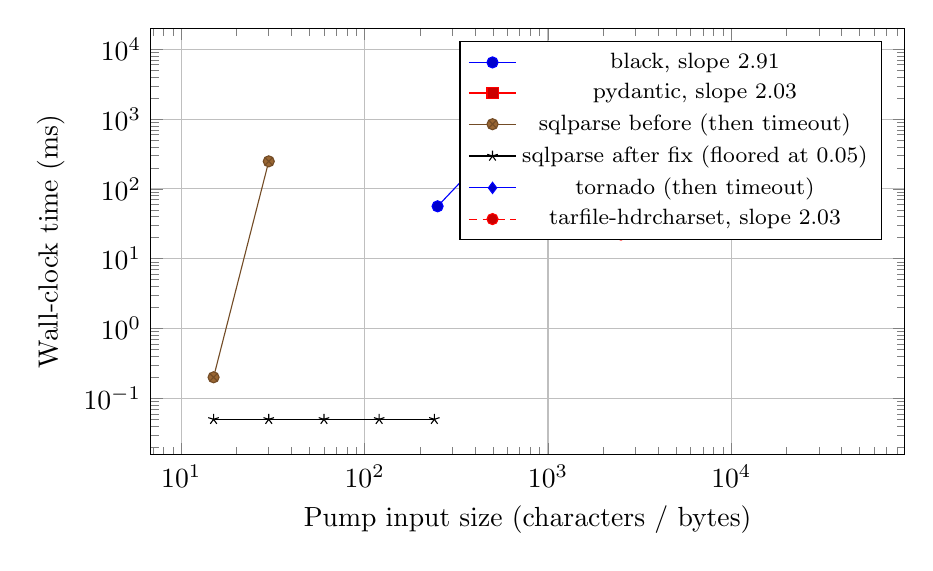
\begin{tikzpicture}
\begin{loglogaxis}[
    width=0.92\textwidth, height=7cm,
    xlabel={Pump input size (characters / bytes)},
    ylabel={Wall-clock time (ms)},
    legend pos=north east,
    legend style={font=\footnotesize},
    grid=major,
]
\addplot coordinates {(250,56.3) (500,385.3) (1000,3173.6)};
\addlegendentry{black, slope 2.91};
\addplot coordinates {(1500,23.2) (3000,84.5) (6000,367.3) (12000,1555.6) (24000,6075.1)};
\addlegendentry{pydantic, slope 2.03};
\addplot coordinates {(15,0.2) (30,248.2)};
\addlegendentry{sqlparse before (then timeout)};
\addplot coordinates {(15,0.05) (30,0.05) (60,0.05) (120,0.05) (240,0.05)};
\addlegendentry{sqlparse after fix (floored at 0.05)};
\addplot coordinates {(5000,336.3) (10000,1286.3) (20000,5110.5)};
\addlegendentry{tornado (then timeout)};
\addplot coordinates {(2500,22.2) (5000,93.4) (10000,399.0) (20000,1503.4) (40000,6200.4)};
\addlegendentry{tarfile-hdrcharset, slope 2.03};
\end{loglogaxis}
\end{tikzpicture}
\caption{Measured growth curves (log-log). Series stop where the 15\,s timeout fires. The fixed sqlparse series is flat at the measurement floor. The tarfile-pax control ($\le$0.4\,ms, slope 0.93) is omitted as a flat line at the bottom.}
\label{fig:growth}
\end{figure}

\subsection{sqlparse: proven fix}

The vulnerable string pattern times out from size 60 upward. The atomic-star rewrite commits the alternation to its greedy first path and re-times at $\le$0.1\,ms on all five sizes (linear), with all four advisory-derived accepts and both rejects byte-identical. This is the headline: an exponential CVE pattern repaired by a mechanical atomic-group rewrite, proven by measurement rather than argued by inspection.

\subsection{black and pydantic: honestly unfixed}

Black's pattern is genuinely exponential (slope 2.91, timeouts from size 2000), but no rule in the v1 set applies soundly: the obvious atomic rewrite of the whitespace prefix changes benign verdicts (atomic whitespace cannot backtrack onto the tab run), so the accept-rule correctly rejects it---and upstream itself removed the regex rather than repairing it. Pydantic's pattern is cleanly quadratic (slope 1.99--2.03, $\sim$4.2$\times$ per doubling), but atomic treatment of the lazy group breaks valid addresses, so it stays unfixed; upstream capped input length instead. Both entries document the cause rather than hiding behind a weaker claim.

\subsection{tornado and tarfile: usage-level lessons}

Tornado's case is not one evil pattern but a quadratic \textit{usage}: two cheap patterns re-searched from a moving index inside a while loop (311\,ms at 20k doubling to timeout at 100k, matching upstream's ``over a minute'' report). No pattern-level rewrite can fix a loop; the fix is structural (single substitution pass, as upstream shipped). The tarfile pair splits instructively: the PAX single-match is linear (slope 0.93) despite its suspect shape---kept as a negative control proving the harness does not cry wolf---while the hdrcharset \textit{search} is quadratic (slope 2.00), because search-mode rescans from every start position. That asymmetry is the report's sharpest lesson: in search mode, the position scan dominates, not the per-position backtrack.

\section{Discussion}
\label{sec:discussion}

\subsection{Key findings}

First, measurement settles what inspection cannot: six suspect-shaped patterns resolve into two exponential, three polynomial, and one linear case, with fitted exponents (0.76--3.05) landing exactly on their theoretical classes. Second, the fix loop works where the theory says it should (alternation overlap in sqlparse) and refuses where it should not (black, pydantic), which is the accept-rule doing its job---a rewriter that never says no is a liability. Third, two upstream fixes confirm our framing from the other direction: where we report UNFIXED, upstream authors also declined to repair the pattern (removal, caps, restructures).

\subsection{Advisory prose is unreliable}

The published vendor proof-of-concept for the pydantic CVE (\verb!'<' + ' ' * 3000!) measures 0.0\,ms on CPython 3.12---it does not reproduce. Our spaces-first pump does (92\,ms at 3000 growing quadratically to 1.5\,s at 12000). Vendor pages in this space reuse templated explainer text across CVEs; the corpus policy of extracting patterns from fix diffs and reproducing locally before freezing exists because of exactly this finding.

\subsection{Possessive quantifiers are not a general fix}

A third rewrite rule (leading digit-run to possessive) was prototyped for the tarfile-hdrcharset case. It passed benign checks but delivered only a constant-factor win (18\,ms vs 29\,ms at size 2500) with the complexity class unchanged: in search mode the per-position scan dominates regardless of per-position backtracking. The rule was deleted. This negative result is reported because it is the kind of plausible-sounding fix the report's own framework exists to reject.

\subsection{Limitations}

Pump strings are synthetic, not traffic replays; adversarial inputs in the wild may shape differently. The 15\,s timeout and five-size sweeps are judgment calls, documented in code. Benign sets are small (strongest for sqlparse at 4+2, thinnest elsewhere)---acceptable for a fix-gate, insufficient for a generality claim, which is why none is made. Only CPython 3.12 on one machine is measured; engine-version variance is untested. The corpus is six entries: a benchmark, not a census.

\subsection{Future work}

In priority order, as filed in the repository's contributing guide: (1) a parser-replacement table benchmarking email-validator and urllib.parse drop-ins with measured false-accept/reject rates; (2) pump knee-tuning per entry; (3) benign-set expansion from advisory tests for tornado and black; (4) new rewrite rules behind the unchanged accept-rule gate.

\section{Conclusion}

On a frozen corpus of six entries across five real CVEs, a 184-line standard-library harness with a strict measure-rewrite-prove loop fixes one exponential pattern with timing proof, correctly clears one linear control, measures one driver-level quadratic, and reports four cases unfixed with evidenced causes. The work's secondary contribution is methodological: reproduce advisories locally before trusting them, record timeouts as data, and let a conjunction of identical benigns plus linear re-measurement---not inspection---decide what counts as fixed.

\section{Reproducibility}
\label{sec:repro}

\subsection{Installation}

No dependencies beyond CPython $\ge$ 3.11 (atomic-group syntax does not exist below) and pytest for the suite. Clone and run; nothing is downloaded, compiled, or installed.

\subsection{Run benchmarks}

\begin{lstlisting}[language=bash]
git clone https://github.com/AshayK003/redos-harness.git
cd redos-harness
python -m pytest tests -q   # 4 passed: evil flagged+fixed, safe clean
python report.py            # regenerates Table 2 and Figure 1
\end{lstlisting}

The suite's canonical pair is \verb!(a+)+$! (must flag exponential and be fixed by rewrite) versus \verb!a+$! (must stay clean), plus a benign-preservation check on every rewrite candidate.

\subsection{Repository structure}

\verb!corpus.json! (frozen v1 measurements and advisory links), \verb!harness.py! (timing, fitting, benign checks), \verb!rewriter.py! (two conservative rules), \verb!report.py! (one-command table), \verb!tests/! (the runnable check), \verb!internals/! (working notes, not published except this report).

\begin{thebibliography}{9}

\bibitem{sok} Bhuiyan et al. \textit{SoK: A Literature and Engineering Review of Regular Expression Denial of Service (ReDoS).} ASIACCS 2025. \url{https://arxiv.org/abs/2406.11618} Artifact: \url{https://github.com/PurdueDualityLab/SoKReDoS-ASIACCS25}

\bibitem{redoshunter} Li et al. \textit{ReDoSHunter: A Combined Static and Dynamic Approach for Regular Expression DoS Detection.} USENIX Security 2021. \url{https://www.usenix.org/system/files/sec21-li-yeting.pdf}

\bibitem{regulator} McLaughlin et al. \textit{Regulator: Dynamic Analysis to Detect ReDoS.} USENIX Security 2022. \url{https://www.usenix.org/system/files/usenixsecurity22-mclaughlin.pdf}

\bibitem{revealer} Zhang et al. \textit{REVEALER: Detecting and Exploiting Regular Expression Denial-of-Service Vulnerabilities.} IEEE S\&P 2021.

\bibitem{rogers} Rogers, J. \textit{A Comparison of Tools to Detect ReDoS-vulnerable Expressions.} 2025. \url{https://joshua.hu/comparing-redos-detection-tools}

\bibitem{py311} CPython 3.11 \textit{re} documentation: atomic grouping and possessive quantifiers (bpo-433030). \url{https://docs.python.org/3.11/library/re.html}

\bibitem{cve6232} CVE-2024-6232 (CPython tarfile). Fix: \url{https://github.com/python/cpython/commit/34ddb64d088dd7ccc321f6103d23153256caa5d4}

\bibitem{cve3772} CVE-2024-3772 (pydantic). Fix: \url{https://github.com/pydantic/pydantic/commit/59d8f38fd6220e3917c53785dbc70317d6f8e631}

\bibitem{cve30608} CVE-2023-30608 (sqlparse). Fix: \url{https://github.com/andialbrecht/sqlparse/commit/c457abd5f097dd13fb21543381e7cfafe7d31cfb}

\bibitem{cve52804} CVE-2024-52804 (tornado). Fix: \url{https://github.com/tornadoweb/tornado/commit/d5ba4a1695fbf7c6a3e54313262639b198291533}

\bibitem{cve21503} CVE-2024-21503 (Black). Advisory: \url{https://github.com/advisories/GHSA-fj7x-q9j7-g6q6}

\end{thebibliography}

\end{document}
